

\documentclass[a4paper, 10pt, spanish]{article}
\usepackage{color}
\definecolor{cadet}{rgb}{0.33, 0.41, 0.47}
\definecolor{orange}{rgb}{0.93, 0.53, 0.18}
\definecolor{carminered}{rgb}{1.0, 0.0, 0.22}
\definecolor{green}{rgb}{0.33, 0.42, 0.18}
\definecolor{darkmagenta}{rgb}{0.55, 0.0, 0.55}
\usepackage{anysize}
\usepackage{amsmath}
\usepackage{biblatex}
\usepackage{float}
\usepackage{array} % 1
\usepackage{graphicx}
\usepackage{tikz}
\usetikzlibrary{calc,patterns,angles,quotes}
\usetikzlibrary{calc,decorations.pathmorphing,patterns}
\usepackage{graphicx}
\usepackage[spanish]{babel}
\usepackage[T1]{fontenc}
\usepackage[utf8]{inputenc}
\usepackage{textcomp}
\usepackage{fancyhdr}
\usepackage{color}
\usepackage{courier}
\usepackage{multirow}
\usepackage{float}
\usepackage{listings}
\usepackage{pgfplots,filecontents}
\pgfplotsset{compat=1.7}
\pgfplotsset{compat=newest}
\usepgfplotslibrary{units}
\usepackage[siunitx]{circuitikz}
\usepackage{caption}
\usepackage{subcaption}
\usepackage{cleveref}
\usepackage{tabularx}
\usepackage{lscape}
\usepackage{pdflscape}
\usepackage{booktabs}


\usepackage{lastpage}   % Para poder saber cuántas páginas tiene el documento
\pagestyle{fancy}
\renewcommand{\sectionmark}[1]{\markboth{}{\thesection\ \ #1}}
\fancyhead{}	% Elimino el contenido del encabezado
% El siguiente texto a la derecha (izquierda) en páginas pares (impares)
\fancyhead[RE,LO]{86.06 - Circuitos Electrónicos - Informe N\textsuperscript{o}2}
\fancyhead[R]{FIUBA}

\fancyfoot{}	% Elimino el contenido del pie de página
% A la izquierda (derecha) en páginas pares (impares): nro. de página / total
\fancyfoot[LE,RO]{\thepage/\pageref{LastPage}}



\begin{document}


\marginsize{2cm}{2cm}{2cm}{2cm}
%
% Carátula:
%
\begin{titlepage}

\thispagestyle{empty}

\begin{center}

\includegraphics[scale=0.3]{fiuba.pdf}\\
\large{\textsc{Universidad de Buenos Aires}}\\
\large{\textsc{Facultad de Ingeniería}}\\
% Modificar año y cuatrimestre
\small{Año 2019 - 2\textsuperscript{o} cuatrimestre}
\end{center}

\vfill

\begin{center} % Modificar el código de ser necesario
\Large{\underline{\textsc{Circuitos Electrónicos (86.06)}}}\\ \vspace{0.5cm}
\Large{\underline{\textsc{Etapas con Transistores Integrados}}}\\ \vspace{0.5cm}
\Large{\underline{\textsc{Informe de Laboratorio N\textsuperscript{o}~3}}}
\end{center}

\vfill

\begin{center}
\large{José F. González - 100063 - \footnotesize{\verb!<jfgonzalez@fi.uba.ar>!}}\\ \vspace{0.25cm}
\large{Gottfried, Joel - 102498 - \footnotesize{\verb!<joelgottfried99@gmail.com>!}}\\\vspace{0.25cm}
\large{Urquiza, Elias - 100714 - \footnotesize{\verb!<eurquiza@fi.uba.ar>!}}\\
\end{center}

\vfill

\hrule
\vspace{0.2cm}

% Modificar código de ser necesario
\noindent\small{86.06 - Circuitos Electrónicos \hfill }

\end{titlepage}

%
% Hago que las páginas se comiencen a contar a partir de aquí:
%
\setcounter{page}{1}

%
% Pongo el índice en una página aparte:
%
\tableofcontents
\newpage


\section{Objetivos}
  \begin{itemize}
    \item Analizar las características principales de una etapa amplificadora formada por un MOSFET de doble gate BF966, que puede configurarse como un circuito equivalente de dos transistores NMOSFET de canal preformado.
    \item Comparar los resultados obtenidos mediante el cálculo analítico, la medición en laboratorio y la verificación por simulación con LTSPICE.
  \end{itemize}

\section{Desarrollo}

\section{Cálculo Analítico}

Utilizando el modelo presente en la fig. \ref{fig:circuito}, calculamos analíticamente los valores de reposo y los parámetros de señal para frecuencias medias.

\begin{center}
  \begin{circuitikz}
              \ctikzset{resistor = european}
              \draw
              (0, 0) node[nigfete] (fet1) {}
              (fet1.G) -- ++ (0,0) to[short,-*] ++(-2,0) node (A) {} to[short,-o] ++ (-1,0) node[left] {\textcolor{red}{$v_{i}$}}
              (A) to[R] ++(0,-4) node[ground] (RG) {}
              (RG) ++ (0.75,1.5) node {$R_G$}
              (fet1.B) -- ++ (fet1.S) to [short,-*] ++ (0,-1.5) node (B) {} to[R] ++(0,-2) node[ground] {}
              (B) ++ (0.75,-0.5) node {$R_S$}
              (B) to[short,-*] ++ (3,0) node(D) {} to[C] ++ (0,-2)  node(C) {} node[ground] {}
              (C) ++ (0.75,1.5) node {$C_G$}

              (4,2) node[nigfete] (fet2) {}
              (D) to (fet2.G)
              (fet1.B) -- ++ (5,0) -- ++ (0,2) to (fet2.B)
              (fet1.D) -- ++ (0,2) -- ++ (4,0)
              (fet2.S) to[short,-*]  ++ (2,0) node(E) {}
              (E) to[R] ++(0,-2) node(F) {} to[american voltage source] ++ (0,-2) node[ground] {}
              (F) ++ (0.75,1.5) node {$R_D$}
              (F) ++ (1,-1.5) node {$V_{CC}$}
              (F) to[short,*-] ++ (2,0) to[C] ++ (0,-2) node[ground] (G) {}
              (G) ++ (0.75,1.5) node {$C_{CC}$}
              (E) to[C] ++(5,0) node (I) {} to[R,*-] ++ (0,-4) node[ground] (H) {}
              (E) ++ (2,1) node {$C_L$}
              (H) ++ (0.75,1.5) node {$R_L$}
              (I) to[short,-o] ++(0.5,0) ++ (0.25,0) node{\textcolor{red}{$v_o$}}
              ;
  \end{circuitikz}
  \captionof{figure}{Esquema simplificado del circuito.}
  \label{fig:circuito}
\end{center}

Se tienen los siguientes datos:
\begin{center}
  \begin{itemize}
    \item $K_1=15\frac{mA}{V^2}$
    \item $K_2=200\frac{mA}{V^2}$
    \item $V_{T_1}=V_{T_2}=V_{T}=-1V$
    \item $\frac{W}{L}=1$
    \item $C_{g_1s} = 2.2pF$
    \item $C_{g_2s} = 1.1pF$
    \item $C_{d_1s} = C_{d_2s} = 0.8pF$
    \item $C_{g_1d} = C_{g_2d} = 25fF$
  \end{itemize}
\end{center}

\subsection{Valores de Reposo}

\begin{center}
  \begin{circuitikz}
              \ctikzset{resistor = european}
              \draw
              (0, 0) node[nigfete] (fet1) {}
              (fet1.G) -- ++ (0,0) to[short,-*] ++(-2,0) node (A) {} to[short,-o] ++ (-1,0) node[left] {\textcolor{red}{$v_{i}$}}
              (A) to[R] ++(0,-4) node[ground] (RG) {}
              (RG) ++ (0.75,1.5) node {$R_G$}
              (fet1.B) -- ++ (fet1.S) to [short,-*] ++ (0,-1.5) node (B) {} to[R] ++(0,-2) node[ground] {}
              (B) ++ (0.75,-0.5) node {$R_S$}
              (B) to[short,-*] ++ (3,0) node(D) {}

              (4,2) node[nigfete] (fet2) {}
              (D) to (fet2.G)
              (fet1.B) -- ++ (5,0) -- ++ (0,2) to (fet2.B)
              (fet1.D) -- ++ (0,2) -- ++ (4,0)
              (fet2.S) to[short,-*]  ++ (2,0) node(E) {}
              (E) to[R] ++(0,-2) node(F) {} to[american voltage source] ++ (0,-2) node[ground] {}
              (F) ++ (0.75,1.5) node {$R_D$}
              (F) ++ (1,-1.5) node {$V_{CC}$}
              ;
  \end{circuitikz}
  \captionof{figure}{Esquema simplificado del circuito de contínua.}
  \label{fig:circuito_continua}
\end{center}

  Planteando la malla de entrada se obtiene
  \begin{equation}
    0 - V_{GSQ_1} - I_D R_S = 0 \Rightarrow -V_{GSQ_1} - R_S K_1 (V_{GSQ_1}-V_{T_1})^2 = 0
  \end{equation}
  Desarrollando el cuadrado de la Ec. 1 se obtiene la siguiente expresión:
  \begin{equation}
    -R_S K_1 V_{GSQ_1}^2  + (2R_S K_1 V_T - 1) V_{GSQ_1} - R_S K_1 {V_{T}}^2 = 0
  \end{equation}
  Por lo que se obtiene
  \begin{equation}
     V_{GSQ_1}=-0.77V \Rightarrow I_{DQ_1}=793.5 \mu A
  \end{equation}

  Debido a que la corriente será la misma en ambos transistores, se pueden despejar los valores de reposo:

  \begin{equation}
    Q_1=(0.94V;793.5\mu A)
  \end{equation}
  \begin{equation}
    Q_2=(4.54V;793.5\mu A)
  \end{equation}

  \begin{equation}
    Q_T=(5.48V;793.5\mu A)
  \end{equation}

\subsection{Análisis de Señal a Frecuencias Medias}

\begin{circuitikz}
\ctikzset{resistor = european}
\draw
(0, 0) node[nigfete] (fet1) {}
(fet1.G) -- ++ (0,0) to[short,-*] ++(-2,0) node (A) {} to[short,-o] ++ (-1,0) node[left] {\textcolor{red}{$v_{i}$}}
(A) to[R] ++(0,-4) node[ground] (RG) {}
(RG) ++ (0.75,1.5) node {$R_G$}
(fet1.B) -- ++ (fet1.S) to [short] ++ (0,-1.5) node (B) {} to[short] ++(0,-2) node[ground] {}
(B)  ++ (3,0) node(D) {} to[short] ++ (0,-2)  node(C) {} node[ground] {}


(4,2) node[nigfete] (fet2) {}
(D) to (fet2.G)
(fet1.B) -- ++ (5,0) -- ++ (0,2) to (fet2.B)
(fet1.D) -- ++ (0,2) -- ++ (4,0)
(fet2.S) to[short,-*]  ++ (2,0) node(E) {}
(E) to[R] ++(0,-2) node(F) {} to[short] ++ (0,-2) node[ground] {}
(F) ++ (0.75,1.5) node {$R_D$}


(E) to[short] ++(5,0) node (I) {} to[R,*-] ++ (0,-4) node[ground] (H) {}

(H) ++ (0.75,1.5) node {$R_L$}
(I) to[short,-o] ++(0.5,0) ++ (0.25,0) node{\textcolor{red}{$v_o$}}
;

\end{circuitikz}

Tenemos los siguientes valores para el análisis:
\begin{center}
   \begin{tabular}{|c|c|c|c|}
     \hline
    Transistor & $g_m$ & $r_{gs}$ & $r_ds$  \\
    \hline
    1 & $6.9\frac{mA}{V}$ & $\rightarrow \infty$ & $\rightarrow \infty$ \\
    \hline
    2 & $25.2\frac{mA}{V}$ & $\rightarrow \infty$ & $\rightarrow \infty$ \\
    \hline
   \end{tabular}
   \captionof{table}{Parámetros de pequeña señal.}
\end{center}

\subsubsection{Amplificación de Tensión Total ($A_v$)}

Si separamos el circuito en dos bloques, uno con amplificación $A_{v1}=v_{o1}/v_i$ y otro con $A_{v2}=v_o/v_{o1}$ como se muestra en el esquema. En las ecuaciones \ref{eq:av1} y \ref{eq:av2} se muestran los resultados.

Para los despejes se utiliza el valor de $r_i^{**}$ que se define en la Ec. \ref{eq:req}. Esta resistencia corresponde a la resistencia equivalente vista desde el Source del segundo transistor hacia el interior de este.

\begin{equation}
  r_i^{**}=\frac{r_{gs_2}}{r_{gs_2} g_{m_2}} = 39.7 \Omega
  \label{eq:req}
\end{equation}

\begin{equation}
  A_{v1}=\frac{v_{o1}}{v_i}=\frac{-i_d r_i^{**}}{\frac{i_d}{g_{m_1} r_{gs}}r_{gs}}=-g_{m_1} r_i^{**} = -0.274
  \label{eq:av1}
\end{equation}

\begin{equation}
  A_{v1}=\frac{v_{o}}{v_{o1}}=\frac{-i_d 2.35K\Omega}{-i_d r_i^{**}}=\frac{2.35K\Omega}{39.7\Omega} = 59.2
  \label{eq:av2}
\end{equation}

Finalmente podemos despejar $A_v$:

\begin{equation}
  A_v=\frac{v_o}{v_i}=\frac{-i_d 2.35k\Omega}{\frac{i_d}{ g_{m_1} r_{gs_1} } r_{gs_1} } = -g_{m_1} 2.35k\Omega = -16.22
  \label{eq:av}
\end{equation}

Que además verifica la relación $A_v = A_{v1} A_{v2}$.

Dado que no tomamos en cuenta ninguna resistencia en serie con la señal del generador, se tiene que $V_i=V_s$ por lo que tenemos:
\begin{equation}
  A_{vs}=A_{v}=-16.22
\end{equation}

\subsubsection{Resistencia de Entrada y de Salida}
Dado que la resistencia del Gate 1 está en paralelo con la resistencia de entrada del transistor, que tiende a infinito por el enunciado, se obtiene:
\begin{equation}
  R_i=1M\Omega // r_{gs_1} = 1M\Omega
\end{equation}

Por otro lado, dado que la resistencia de salida es el paralelo entre la resistencia del drain y la resistencia $r_{ds_2}$, se tiene:

\begin{equation}
  R_{out}=4.7K\Omega // r_{ds_2} = 4.7K\Omega
\end{equation}

\subsubsection{Máxima excursión de señal a la salida sin recorte}

Se estima que existe baja distorsión cuando $\Delta V_{GS} << (V_{GSQ}-V_T)/2$. Esta expresión puede ser justificada al interpretar lo que representa. Dado que $\Delta V_{GS}$ representa la amplitud pico de la señal de entrada, es necesario que la misma no supere el límite para el cual el transistor deja de estar en saturación y entra en modo triodo. Por ello, el limite de la señal de entrada está impuesto por la distancia entre $V_{GSQ}$ y $V_T$. \textcolor{red}\textbf{La distorsión presente, entonces, es la que corresponde a}}

Si se traza la recta de carga dinámica de ambos transistores se pueden observar los límites de amplitud de señal que pueden tener en su salida. Las ecuaciones de ambas rectas de carga se presentan a continuación:


\textbf{\textcolor{red}{INCLUIR LAS RCD}}

\textit{RCD del Primer Transistor:}
\begin{equation}
  i_{D_1} = I_{DQ_1} + \frac{V_{DSQ_1} - v_{d1}}{r_i^{**}} = 24.5mA - \frac{v_{d1}}{39.7\Omega}
\end{equation}
La raíz se encuentra en $v_{D_1} = 973mV$ y la ordenada al origen en $i_{D_1} = 24.5mA$.

\textit{RCD del Segundo Transistor:}
\begin{equation}
  i_{D_2} = I_{DQ_2} + \frac{V_{DSQ_2} - v_{d2}}{4.7K\Omega/2} = 2.73mA - \frac{v_{d1}}{2.35K\Omega}
\end{equation}
La raíz se encuentra en $v_{D_1} = 6.42V$ y la ordenada al origen en $i_{D_1} = 2.73mA$.

La tensión $V_{o1_{max}}= V_{DSQ_1} - 0.94V = 0.97V - 0.94V = 30mV$, mientras que $V_{o_{max}}= V_{DSQ_2} - 4.54V = 6.42V - 4.54V = 1.88V$.

Dado el valor de $A_{V1}$ de la ecuación \ref{eq:av1} se puede despejar la tensión de entrada máxima $v_i$:

\begin{equation}
  v_{i_M}=\frac{30mV}{0.274}=30mV
  \label{eq:in_max_teo}
\end{equation}

Para esta tensión de entrada, por el valor de $A_v$ obtenido en la ec. \ref{eq:av}, se tiene:

\begin{equation}
  v_{o_M}=|A_v|110mV=16.22\ 110mV = 1.8V
  \label{eq:out_max_teo}
\end{equation}

Dado que esta tensión de salida es menor que la obtenida por la RCD del segundo transistor, se puede concluir que el primer transistor es el que limita el comportamiento de esta configuración y los valores presentados en las ecuaciones \ref{eq:in_max_teo} y \ref{eq:out_max_teo} son los valores máximos aproximados que se pueden esperar medir sin recorte.


\subsubsection{Respuesta en frecuencia para $A_{vs}$.}
Con un análisis por inspección podemos obtener un valor aproximado de las frecuencias de corte inferior y superior del sistema. Utilizando el modelo simple propuesto por el enunciado, tenemos los siguientes datos:
\begin{itemize}
  \item $C_{g_1s} = 2.2pF$
  \item $C_{g_2s} = 1.1pF$
  \item $C_{d_1s} = C_{d_2s} = 0.8pF$
  \item $C_{g_1d} = C_{g_2d} = 25fF$
\end{itemize}

Analizando primero la respuesta en bajas frecuencias, considerando entonces únicamente la influencia del capacitor $C_G$, $C_L$, y $C_{cc}$, se calcula lo siguiente:

\textbf{$C_G$:}
\textbf{\textcolor{red}{ESQUEMA}}

\begin{equation}
  \tau_G = (145\Omega//1K\Omega) 1\mu F = 0.127ms \Rightarrow = 1253 Hz
\end{equation}

\textbf{$C_{cc}$:}
\textbf{\textcolor{red}{ESQUEMA}}

\begin{equation}
  \tau_{cc} = 9.4\Omega 0.1\mu F = 0.94ms \Rightarrow = 169 Hz
\end{equation}

\textbf{$C_L$:}
\textbf{\textcolor{red}{ESQUEMA}}

\begin{equation}
  \tau_L = 9.4\Omega 1\mu F = 9.4ms \Rightarrow = 16.9 Hz \approx 170 Hz
\end{equation}

Podemos concluir entonces, dado que la suma de polos ficticios es de $1592Hz$, que la frecuencia de corte inferior tendrá este valor aproximado.

\textcolor{red}{\textbf{[HACER ESQUEMA CIRCUITAL DE ANÁLISIS EN ALTAS FRECUENCIAS AQUÍ]}}

Para el análisis en altas frecuencias, obtenemos los siguientes valores:

\begin{itemize}
  \item $C_{G_1}=2.2pF(1-\frac{v_{source}}{v_i})+25fF(1-\frac{v_o}{v_i}) = 430fF$
  \item $C_{G_2}=1.1pF(1-\frac{v_{source}}{v_{gate_2}}) = 1.1pF$
  \item $C_{D}=25fF(1-\frac{v_i}{v_o})+0.8pF(1-\frac{v_{source}}{v_o}) = 1.3pF$
  \item $C_{Source}=0.8pF(1-\frac{v_o}{v_{source}})+1.1pF(1-\frac{v_{source}}{v_{gate_2}})+2.2pF(1-\frac{v_i}{v_{source}}) = 14.9pF$
\end{itemize}

Obtenemos entonces, sin considerar la capacidad del Gate 2 puesto que el capacitor asociado está en serie con una resistencia equivalente que se considera tiende a infinito:


\textbf{$C_{G1}$:}
\textbf{\textcolor{red}{ESQUEMA}}

\begin{equation}
  \tau_{G1} = 430fF 1M\Omega = 430ns \Rightarrow f_{G1} = 370.1 KHz
\end{equation}


\textbf{$C_{D}$:}
\textbf{\textcolor{red}{ESQUEMA}}

\begin{equation}
  \tau_{D} = 1.3pF 2.35K\Omega = 3.1ns \Rightarrow f_{D} = 51.3 MHz
\end{equation}

\textbf{$C_{S}$:}
\textbf{\textcolor{red}{ESQUEMA}}

\begin{equation}
  \tau_{S} = 14.9 pF 145\Omega = 2.16ns \Rightarrow f_{S} = 73.7 MHz
\end{equation}

Debido a que la frecuencia asociada al Gate 1 es la menor, consideraremos que $f_H=370.1KHz$ es la frecuencia de corte superior del sistema.

\section{Simulación}
Simulando el circuito dado con LTSpice, utilizando el modelo simplificado del integrado, presente en la figura \ref{fig:mod_sim}, verificamos los resultados análiticos calculados en la sección anterior. Consideramos nuevamente los siguientes valores:
\begin{itemize}
  \item $K_1=15\frac{mA}{V^2}$
  \item $K_2=200\frac{mA}{V^2}$
  \item $V_{T_1}=V_{T_2}=V_{T}=-1V$
  \item $\frac{W}{L}=1$
\end{itemize}

\begin{center}
  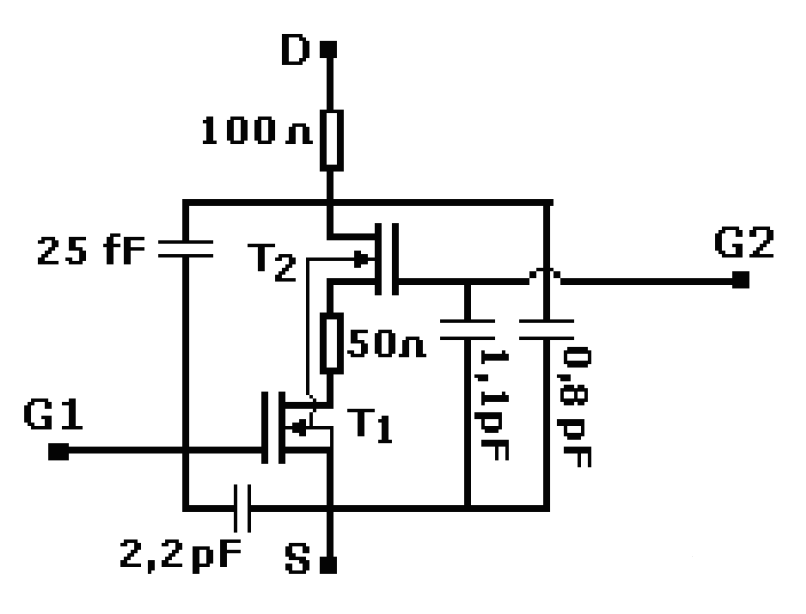
\includegraphics[width=0.5\textwidth]{modelo_simple.png}
  \captionof{figure}{Modelo simple del integrado según lo propuesto por el enunciado.}
  \label{fig:mod_sim}
\end{center}

\subsection{Valores de Reposo}

\begin{center}
  \begin{tabular}{|c|c|c|c|c|}
    \hline
    $V_{G1_Q}$ & $V_{G2_Q}$ & $V_{S_Q}$ & $V_{D_Q}$ & $V_{cc}$ \\
    \hline
    $0V$ & $695mV$ & $695mV$ & $6.73V$ & $10V$ \\
    \hline
  \end{tabular}
  \captionof{table}{Valores de reposo simulados.}
  \label{tab:valores_reposo_sim}
\end{center}

\begin{equation}
  V_{DS_{Q}} = V_{D_Q} - V_{S_Q} = 6V
\end{equation}

\begin{equation}
  I_{DQ} = 695 \mu A
\end{equation}

\subsection{Análisis de Señal a Frecuencias Medias}

\subsubsection{Amplificación de Tensión Total ($A_v$)}
Alimentando al circuito con una señal de entrada de $10mV$ pico y de frecuencia $10KHz$ se obtuvo el gráfico de la figura \ref{fig:Av_sim}. Con el cociente de los valores pico de tensión se puede concluir que $A_v=-10.6$ y $A_{vs}$ tendrá el mismo valor puesto que no estamos considerando algún valor de resistencia en serie con la fuente de señal.

\begin{center}
  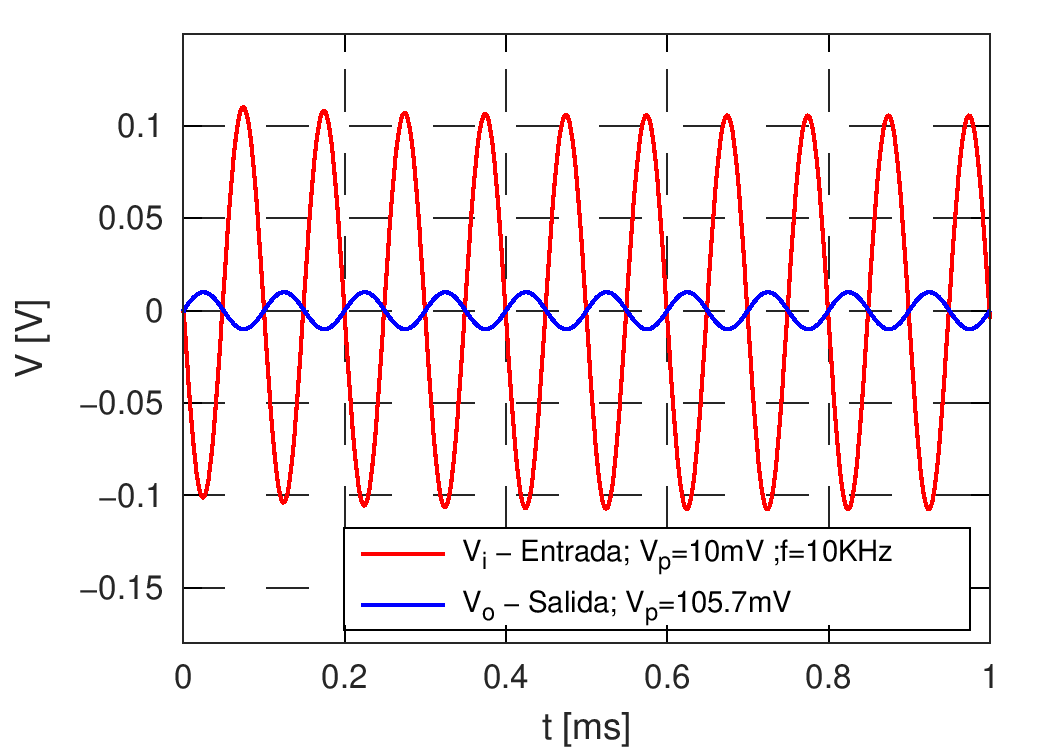
\includegraphics[width=0.7\textwidth]{Av_sim.png}
  \captionof{figure}{Señal de entrada y salida dentro del rango de frecuencias medias obtenida por simulación.}
  \label{fig:Av_sim}
\end{center}

\subsubsection{Resistencia de Entrada y de Salida}
\textbf{Resistencia de Entrada}
Dado que no se registra corriente entrante por el Gate 1, se puede concluir entonces que
\begin{equation}
  R_{in} = 1M\Omega
\end{equation}

\textbf{Resistencia de Salida}
\begin{center}
  \begin{circuitikz}
  \ctikzset{resistor = european}
  \draw

  (0, 0) to[R] ++(0,-2) node(F) {} to[short] ++ (0,-2) node[ground] {}
  (F) ++ (0.75,1.5) node {$R_D$}

  (0, 0) to[short] ++(5,0) node (I) {} to[R,*-] ++ (0,-4) node[ground] (H) {}

  (H) ++ (0.75,1.5) node {$R_L$}
  (I) to[short,-o] ++(0,0.5) ++ (0, 0.25) node{\textcolor{red}{$v^*$}}

  (I) to[R] ++(5,0) node (P) {} ++(-0.25, 0.25) node{$R_p=4.7K\Omega$}

  (P) to[short, -o] ++(1, 0) ++(0.5, 0) ++ (0.25, 0) node{\textcolor{red}{$v_p$}}
  ;

  \end{circuitikz}
\end{center}


Pasivando la fuente de señal entre Gate 1 y común, y colocando una fuente de prueba con $V_{p(pico)}=330mV$ en serie con una resistencia de $4.7K\Omega$ en el nodo e salida del circuito, se puede calcular la $R_{out}$ por medio del análisis siguiente:

\begin{equation}
  \frac{V_p - V^*}{4.7K\Omega} - \frac{V^*}{4.7K\Omega} = i_{R_{out}} = \frac{V^*}{R_{out}}
\end{equation}

Se obtuvo
\begin{equation}
  V^* = 108.9 mV \Rightarrow i_{R_{out}} = 23.9 \mu A \Rightarrow R_{out} = 4.6K\Omega
\end{equation}

\subsubsection{Máxima Excursión de Señal a la salida sin recorte}

\begin{center}
  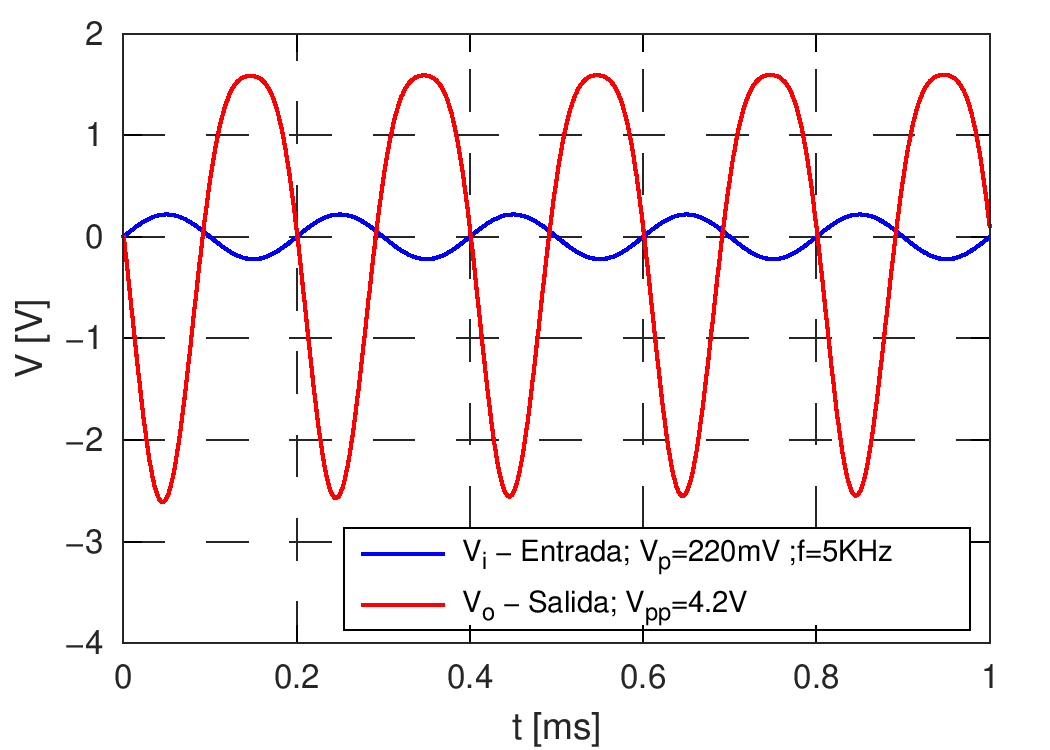
\includegraphics[width=0.7\textwidth]{vomax_sim.png}
  \captionof{figure}{Señal de entrada y salida máxima sin recorte obtenida por simulación.}
  \label{fig:vomax_sim}
\end{center}

Como se observa en la figura \ref{fig:vomax_sim}, se tiene que la tensión de salida máxima sin recorte y con baja distorsión es de $V_{o(max)_{pp}}=4.2V$ para una señal $V_{s_{pp}}=440mV$. Con estos parámetros se utilizó el comando \textbf{.FOURIER} de LTSpice para calcular la TDH, obteniendose así:

\begin{equation}
  TDH=19.93\%
\end{equation}

\begin{center}
  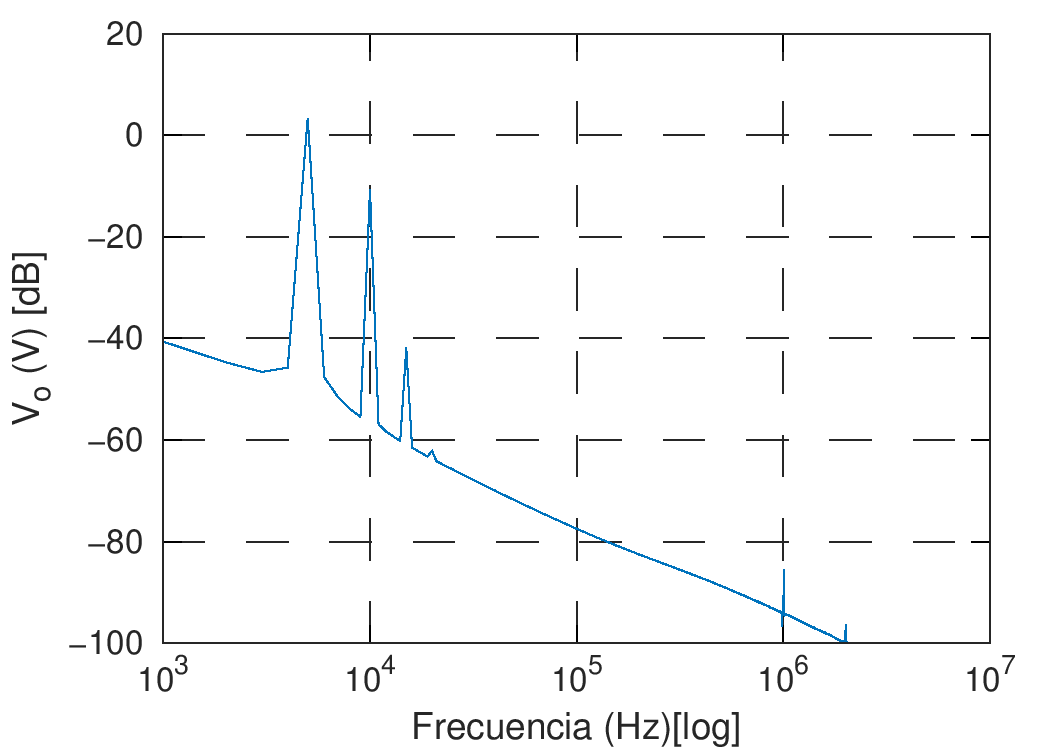
\includegraphics[width=0.7\textwidth]{fft_out.png}
  \captionof{figure}{FFT de la señal de salida presente en la figura \ref{fig:vomax_sim} para la que se obtuvo TDH=19.93\%.}
  \label{fig:fft_sim}
\end{center}

\subsubsection{Respuesta en Frecuencia para $A_{vs}$}

Se simuló la respuesta en frecuencia para cuatro casos distintos: sin simular las puntas del osciloscopio; simulando puntas X1; simulando puntas X10; simulando puntas activas. Se presentan a continuación los resultados obtenidos.

\begin{center}
  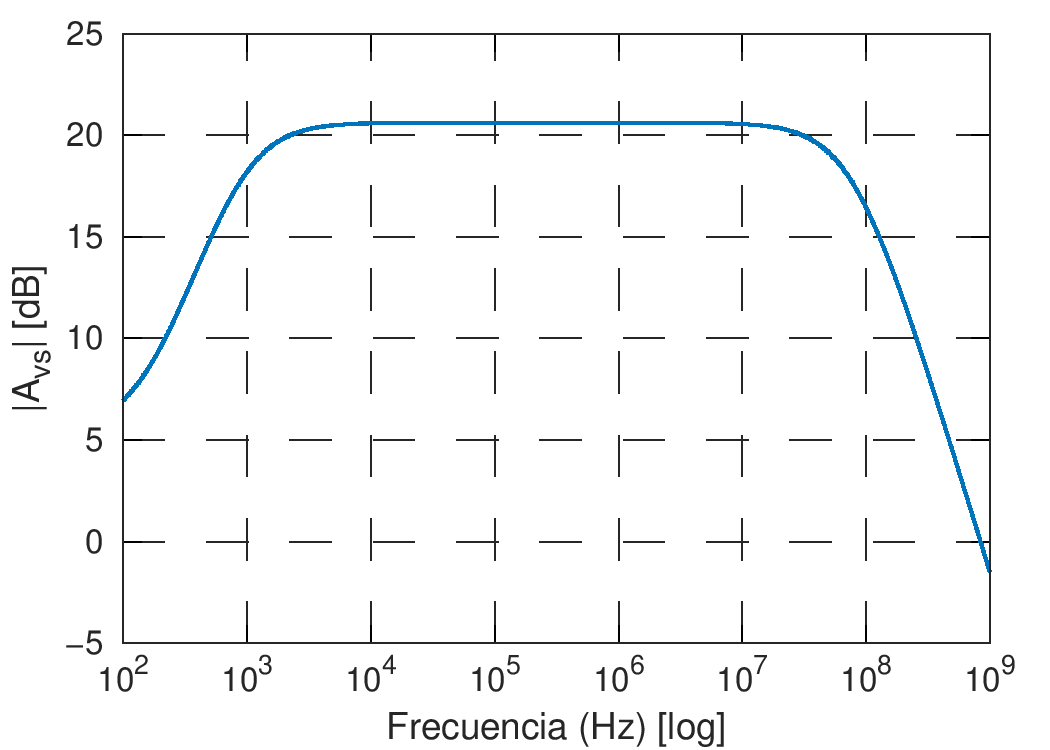
\includegraphics[width=0.7\textwidth]{sim_sin_bode.png}
  \captionof{figure}{Respuesta en frecuencia sin simular puntas de osciloscopio.}
  \label{fig:sim-sin}
\end{center}

\begin{center}
  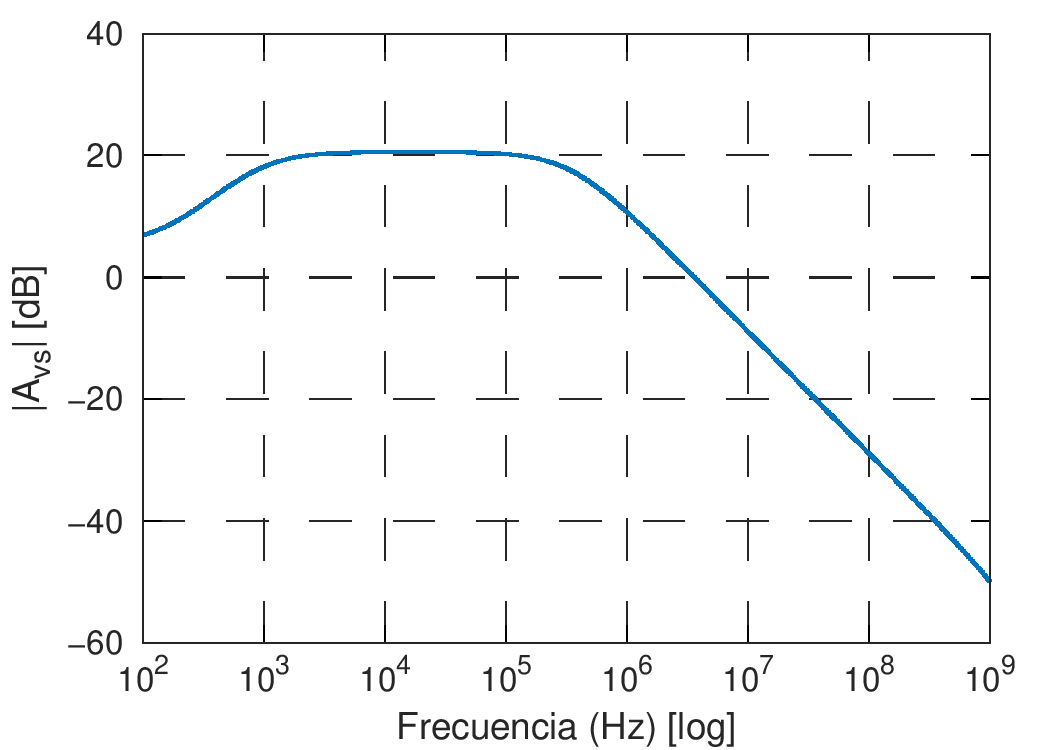
\includegraphics[width=0.7\textwidth]{sim_x1_bode.png}
  \captionof{figure}{Respuesta en frecuencia simulando puntas X1.}
  \label{fig:sim-x1}
\end{center}

\begin{center}
  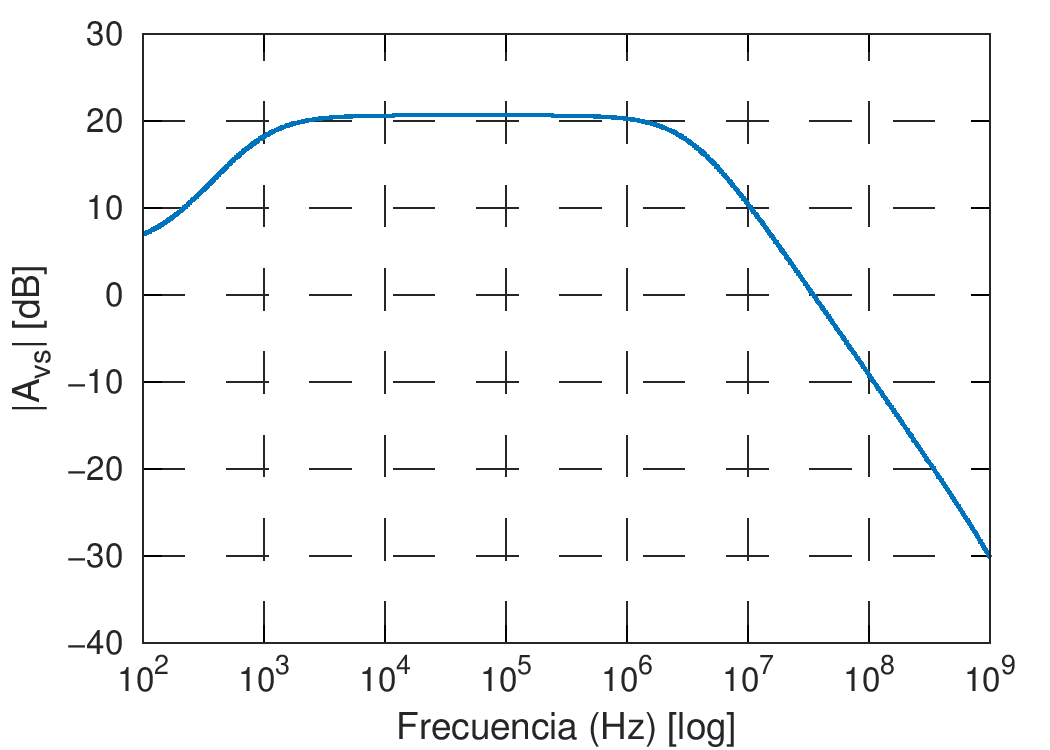
\includegraphics[width=0.7\textwidth]{sim_x10_bode.png}
  \captionof{figure}{Respuesta en frecuencia simulando puntas X10.}
  \label{fig:sim-x10}
\end{center}

\begin{center}
  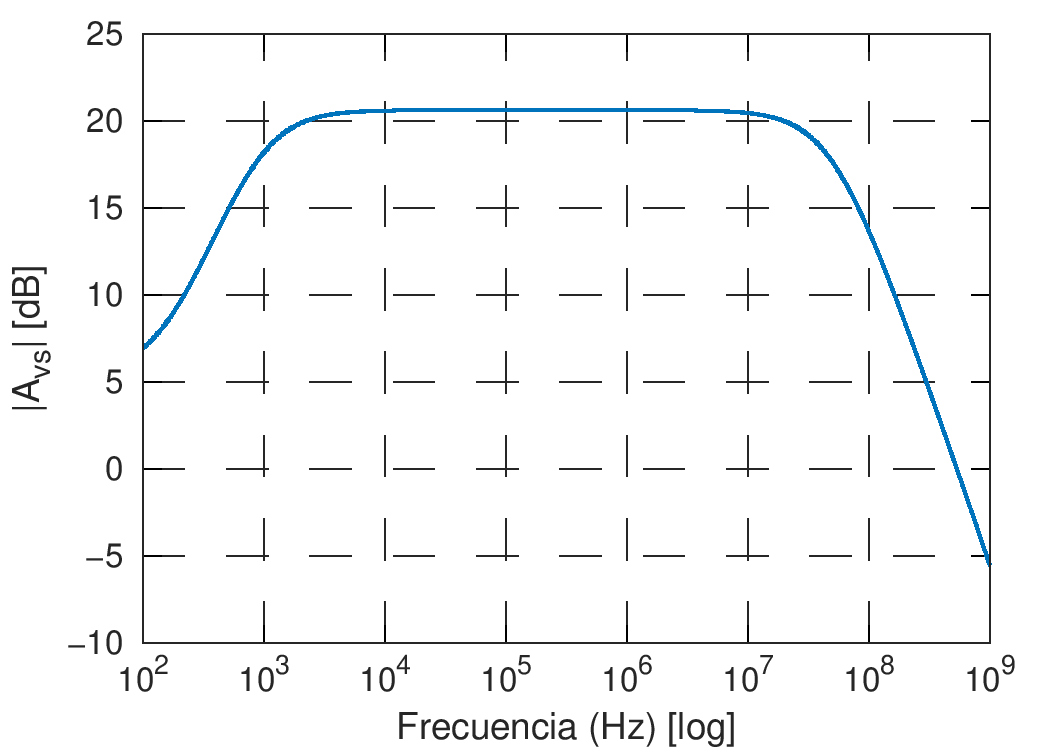
\includegraphics[width=0.7\textwidth]{sim_activa_bode.png}
  \captionof{figure}{Respuesta en frecuencia simulando puntas activas.}
  \label{fig:sim-activa}
\end{center}

Podemos observar que la frecuencia de corte inferior no es alterada apreciablemente con el uso de las distintas puntas de medición, obteniendo entonces:

\begin{equation}
  f_l \approx 3KHz
\end{equation}

Por otro lado, la frecuencia de corte superior se ve disminuida con el uso de puntas X1 y X10 respecto a la obtenida sin simular las puntas. La frecuencia de corte superior que más se asemeja a la $f_h$ es la obtenida utilizando puntas activas, por tener una capacidad mucho menor que las otras dos.

\begin{equation}
  f_h \approx 11MHz
\end{equation}

\section{Mediciones}

\subsection{Valores de Reposo}

\begin{center}
  \begin{tabular}{|c|c|c|c|c|}
    \hline
    $V_{G1_Q}$ & $V_{G2_Q}$ & $V_{S_Q}$ & $V_{D_Q}$ & $V_{cc}$ \\
    \hline
    $4.8mV$ & $700mV$ & $700mV$ & $7.6V$ & $10V$ \\
    \hline
  \end{tabular}
  \captionof{table}{Valores de reposo medidos.}
  \label{tab:valores_reposo_med}
\end{center}

\begin{equation}
  V_{DS_Q} = 6.9V
\end{equation}

\begin{equation}
  I_{DQ} = \frac{V_{cc} - V_{D_Q}}{R_D} = \frac{10V - 7.6V}{4.7K\Omega} = 511 \mu A
\end{equation}

\subsection{Análisis de Señal a Frecuencias Medias}

\subsubsection{Amplificación de Tensión Total ($A_v$)}

\textbf{\textcolor{red}{GRAFICAR Vi y Vo EN UN SOLO GRÁFICO}}
\begin{center}
  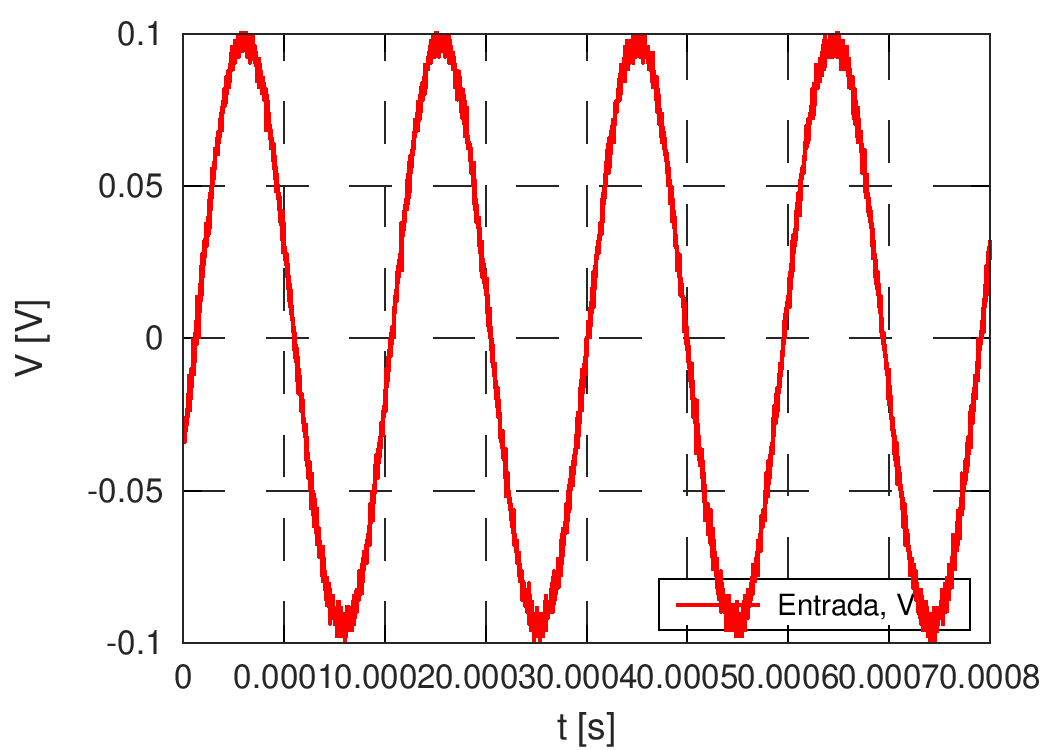
\includegraphics[width=.5\textwidth]{vi.png}
  \captionof{figure}{Señal de entrada.}
  \label{fig:vi_med}
\end{center}

\begin{center}
  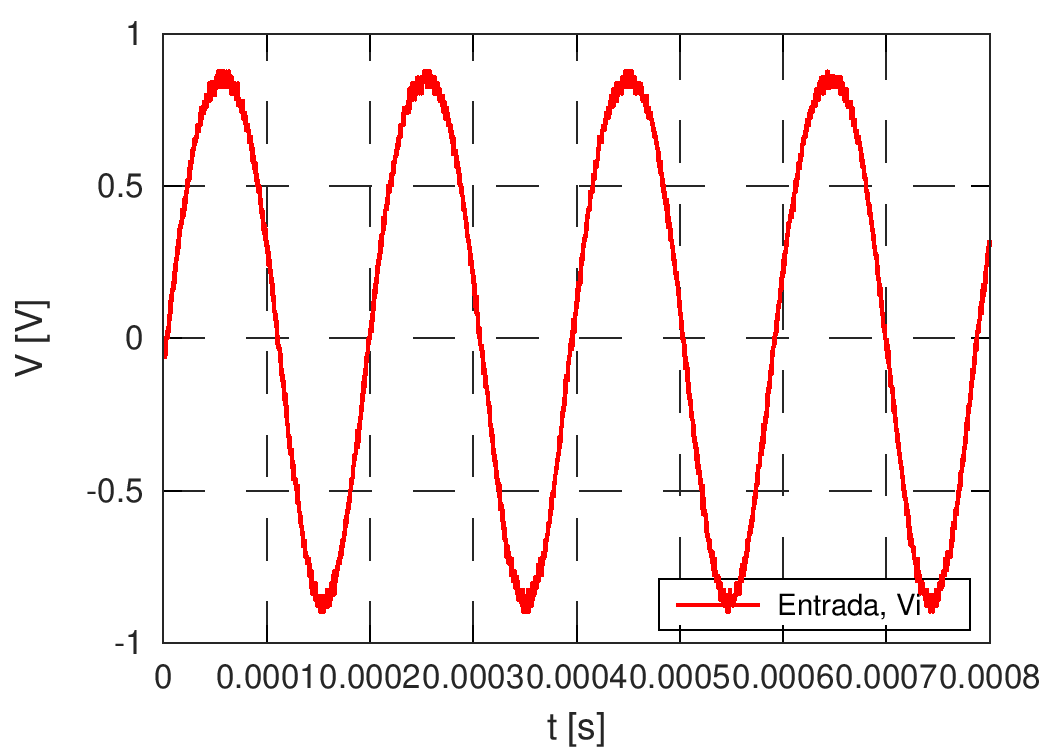
\includegraphics[width=.5\textwidth]{vo.png}
  \captionof{figure}{Señal de salida.}
  \label{fig:vo_med}
\end{center}


\begin{equation}
  A_v=\frac{1.8V_{pp}}{200mV_{pp}}=9
\end{equation}

\subsubsection{Resistencia de Entrada y de Salida}
\textbf{Resistencia de Entrada:}
Dado que la tensión de reposo en el Gate 1 es cercana a 0V, consideramos que la resistencia de entrada se corresponde a $R_G$ tal que:

\begin{equation}
  R_{in}=1M\Omega
\end{equation}

\textbf{Resistencia de Salida}
Colocando una resistencia de prueba de $R_p = 4.7K\Omega$ sobre la carga junto con una tensión de prueba $V_p$ se obtuvo:

\begin{equation}
  V_p= 660mV_{pp} \Rightarrow V^*_{(R_L//R_{out})} = 244 mV_{pp}
\end{equation}

Con este valor podemos despejar $(R_L//R_{out})$:
\begin{equation}
  V^*=V_p \frac{(R_L//R_{out})}{R_p + (R_L//R_{out})} \Rightarrow (R_L//R_{out}) = \frac{V^*\ R_p}{V_p-V^*} = 2.76K\Omega
\end{equation}

\begin{equation}
  \frac{R_{out}R_L}{R_{out}+R_L} = (R_L//R_{out})  \Rightarrow R_{out}=\frac{(R_L//R_{out}) R_L}{R_L - (R_L//R_{out})}
\end{equation}

\begin{equation}
  R_{out}=\frac{2.76K\Omega\ 4.7K\Omega}{4.7K\Omega - 2.76K\Omega}=6.7K\Omega
\end{equation}

\subsubsection{Máxima excursión de señal a la salida sin recorte}
\textbf{\textcolor{red}{GRAFICAR Vi y Vo EN UN SOLO GRÁFICO. Ese desfasaje no me gusta. creo que no medimos en frecuencias medias.}}
Al medir la máxima excursión sin recorte admitiendo baja distorsión, con una frecuencia de \textbf{5KHz}, obtuvimos la respuesta presente en la figura \ref{fig:vo_exc_med}. La señal de entrada se observa en la figura \ref{fig:vi_exc_med}. Observamos que la máxima tensión pico de entrada es de aproximadamente $V_i=212mV$ obteniendo así una señal de salida alineal de aproximadamente $1.82V$.

\begin{center}
  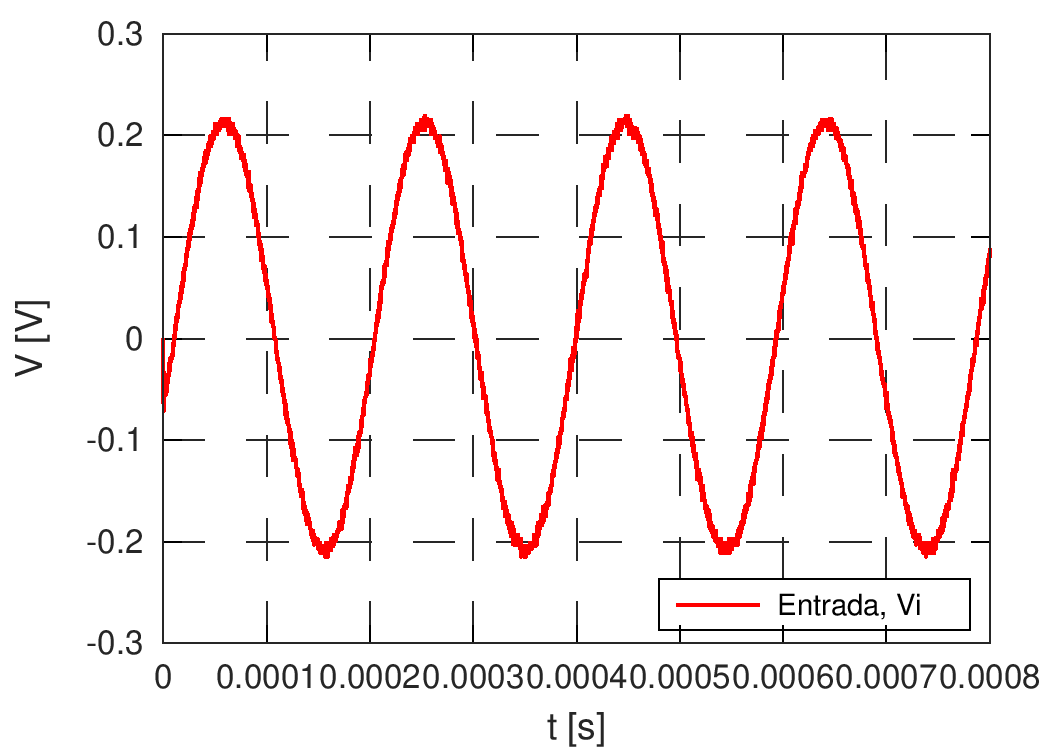
\includegraphics[width=0.5\textwidth]{vi3.png}
  \captionof{figure}{Señal de entrada máxima sin recorte.}
  \label{fig:vi_exc_med}
\end{center}

\begin{center}
  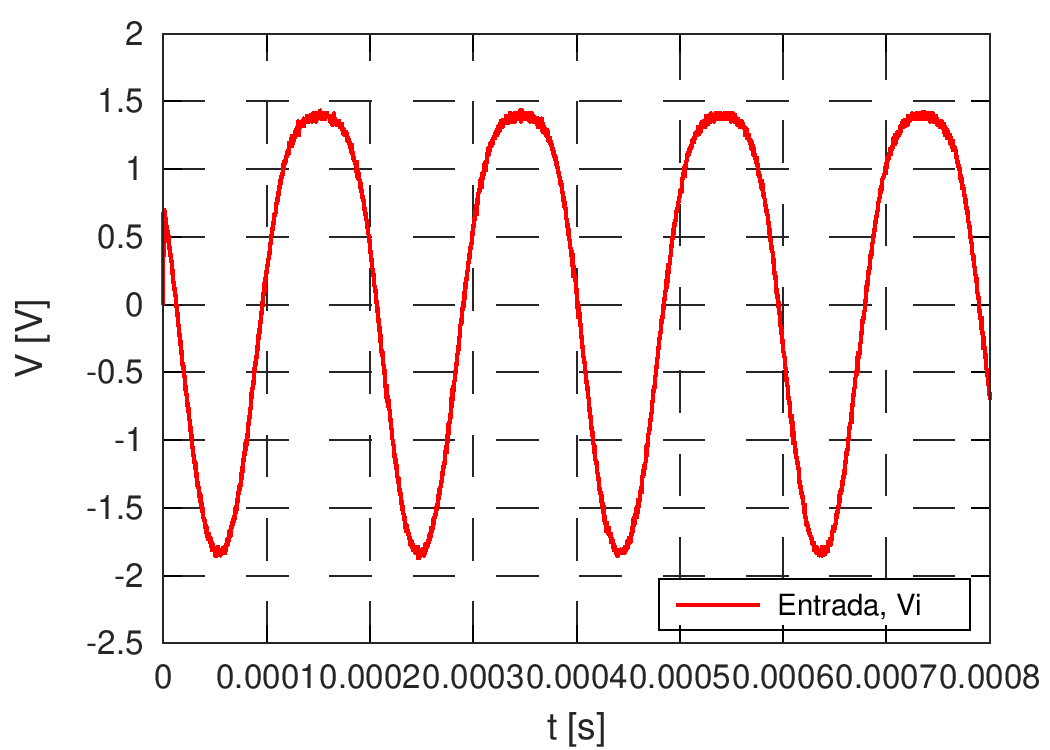
\includegraphics[width=0.5\textwidth]{vo3.png}
  \captionof{figure}{Señal de salida máxima sin recorte.}
  \label{fig:vo_exc_med}
\end{center}

Para evaluar la distorsión de la señal, se utilizó la función FFT del osciloscopio digital, obteniéndose el resultado de la figura \ref{fig:fft_med}.

\begin{center}
  \includegraphics[width=0.5\textwidth]{FFT_MED.png}
  \captionof{figure}{FFT de la señal de salida en su máxima excursión sin recorte. \textbf{Escala: 2.5KHz/div.}}
  \label{fig:fft_med}
\end{center}

Se observa que la señal fundamental es de 5KHz, correspondiente a la frecuencia de la señal de entrada, pero se encuentran otros armónicos de menor magnitud en 10KHz, 15KHz y 20KHz. Estos armónicos indican que la señal de salida no es pura y tenemos un cierto nivel de distorsión presente.

\subsubsection{Respuesta en frecuencia para $A_{vs}$.}
Para medir la respuesta en frecuencia, con una tensión de entrada $V_{s_p}=180mV$, se realizó un barrido de frecuencia hasta 10MHz con puntas pasivas X1, X10, y puntas activas X10 alimentadas por una tensión continua de 9V. Los diagramas de bode realizados con las mediciones se encuentran a continuación. En la tabla \ref{tab:rta_frec_med} se comparan los resultados obtenidos.

\begin{center}
  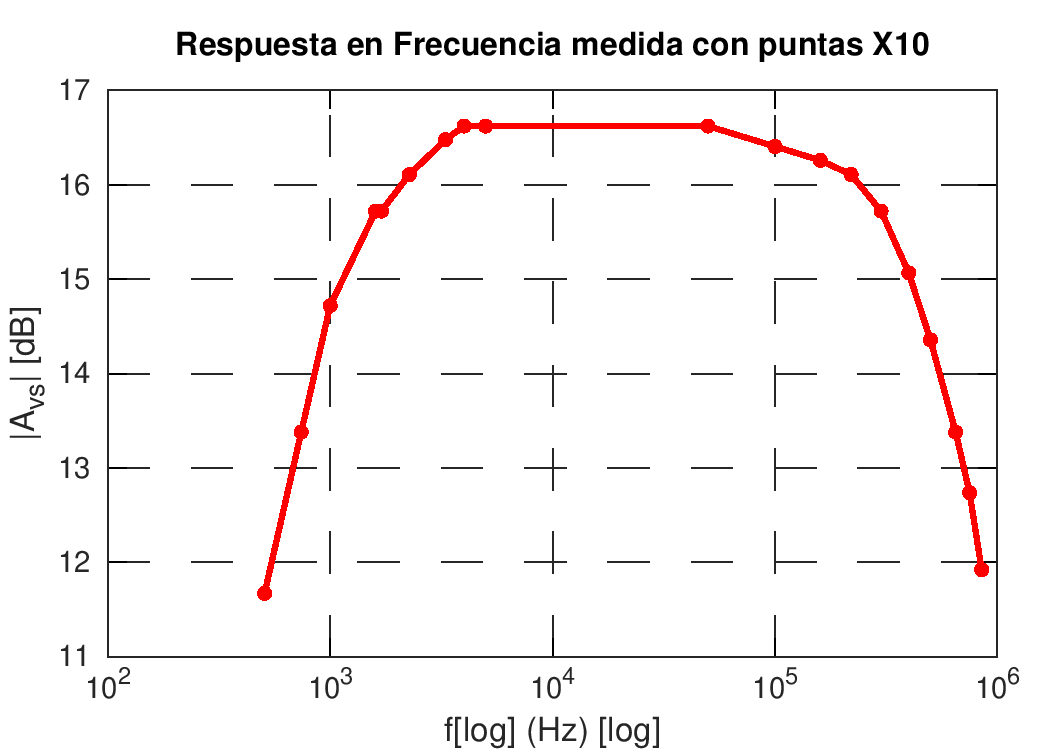
\includegraphics[width=0.8\textwidth]{X1.png}
  \captionof{figure}{Respuesta en frecuencia medida con puntas de osciloscopio X1.}
  \label{fig:X1_med}
\end{center}

\begin{center}
  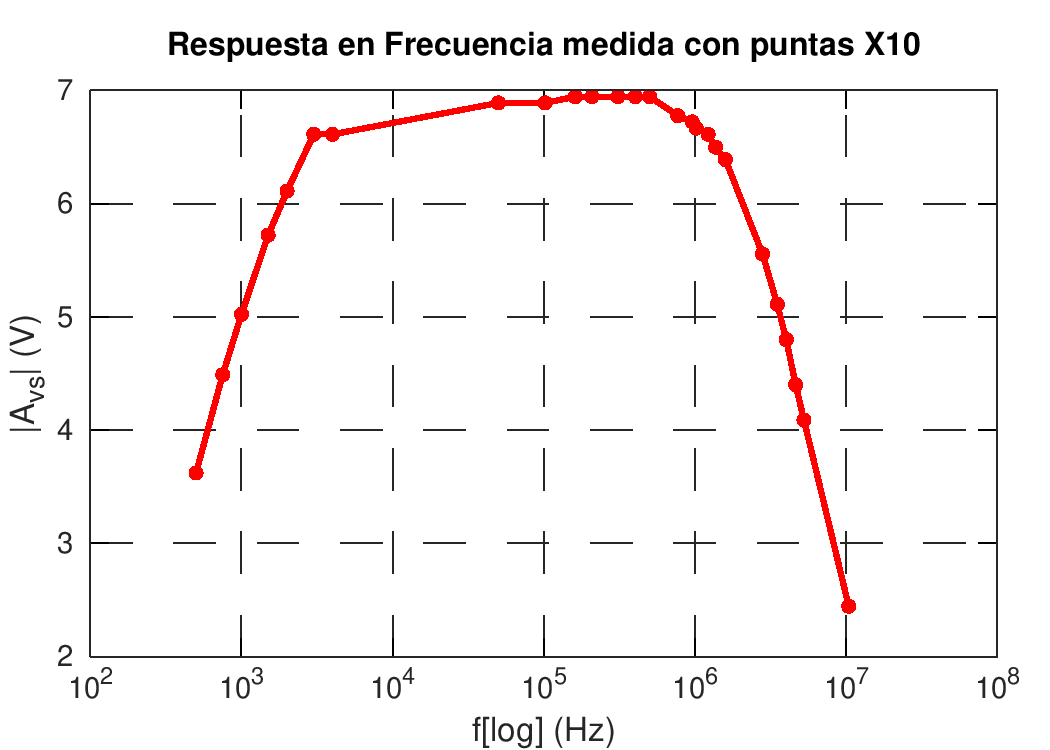
\includegraphics[width=0.8\textwidth]{X10.png}
  \captionof{figure}{Respuesta en frecuencia medida con puntas de osciloscopio X10.}
  \label{fig:X10_med}
\end{center}

\begin{center}
  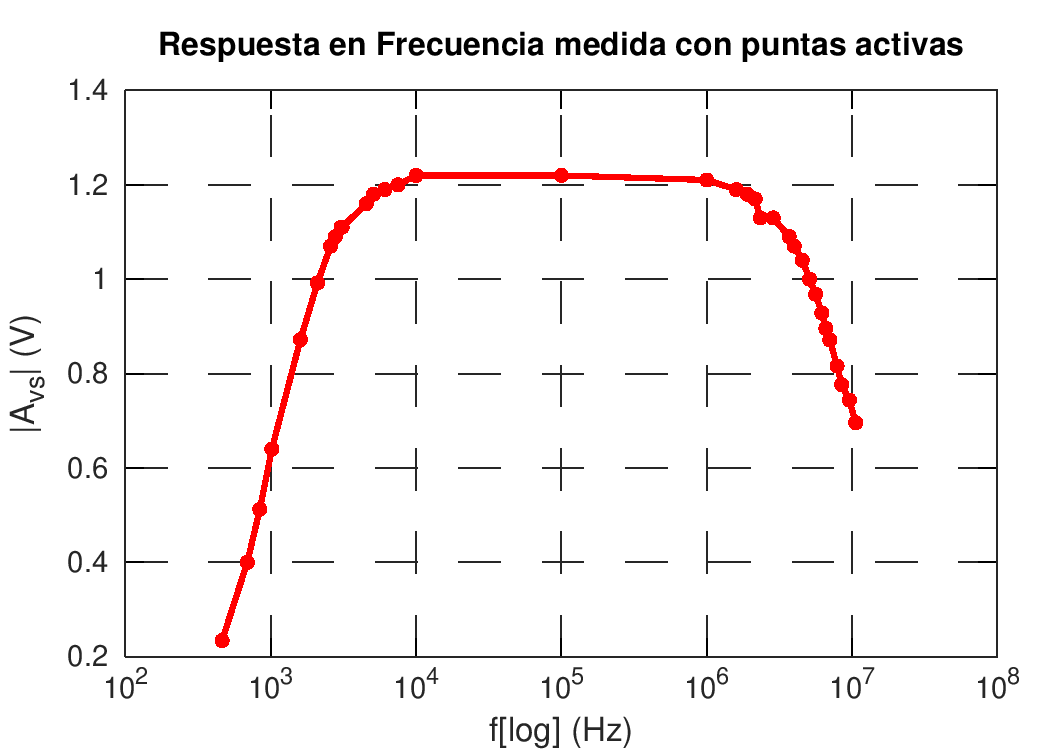
\includegraphics[width=0.8\textwidth]{activas.png}
  \captionof{figure}{Respuesta en frecuencia medida con puntas de prueba activas.}
  \label{fig:activas_med}
\end{center}

\begin{center}
  \begin{tabular}{|c|c|c|c|}
    \hline
    Puntas & $f_l$ & $f_h$ & $|A_{vs}|$ \\
    \hline
    X1 & ~4KHz & ~50KHz & 6.8 \\
    \hline
    X10 & ~3KHz & ~50KHz & 6.9 \\
    \hline
    Activas & ~10KHz& ~100KHz & 6.8 \\
    \hline
  \end{tabular}
  \captionof{table}{Tabla comparativa de los valores de frecuencia de corte inferior y superior. Se incluye también el valor de $|A_{vs}|$.}
  \label{tab:rta_frec_med}
\end{center}

\section{Análisis Comparativo}
En el cuadro \ref{tab:comparativo} se comparan los parámetros de interés. Para el caso de la respuesta en frecuencia medida en el laboratorio, se consideró la frecuencia de corte inferior medida con las puntas X1, por tener más puntos que las mediciones de puntas pasivas X10, y para el valor de la $f_h$ se utilizó aquel obtenido con el uso de puntas de prueba activas, ya que poseen una capacitancia mucho menor que las pasivas y atenúa la influencia de dichas puntas. El error relativo incluido en el cuadro corresponde a la diferencia porcentual entre el valor medido y el analítico, tomando el medido como valor real.

\begin{center}
  \begin{tabular}{|c|c|c|c|c|c|c|c|c|c|}
    \hline
    Valor & $I_{DQ}$ & $V_{DSQ}$ & $A_v$ & $A_{vs}$ & $R_{in}$ & $R_{out}$ & $V{o_{max}}$ & $f_l$ & $f_h$ \\
    \hline
    Analítico & $793.4\mu A$& $5.48V$& -16.22 & -16.22 & $1M\Omega$ & $4.7K\Omega$ & $1.8V$ & $1592Hz$ & $370.1KHz$ \\
    \hline
    Simulado & $695\mu A$ & $6V$ & -10.6 & -10.6 & $1M\Omega$ & $4.6K\Omega$ & $2.15V$ & $3KHz$ & $11MHz$ \\
    \hline
    Medido & $511\mu A$ & $6.9V$ & -9 & -6.8 & $1M\Omega$ & $6.7K\Omega$ & $1.82V$ & $4KHz$ & $100KHz$ \\
    \hline
    \hline
    $\epsilon_{r\%}$ & 55\% & 21\% & 80\% & 105\% & 0\% & 30\% & 1\% & 60\% & 270\% \\
    \hline
  \end{tabular}
  \captionof{table}{Cuadro comparativo de todos los valores obtenidos por análisis, simulación, y medición.}
  \label{tab:comparativo}
\end{center}


        %\section{Referencias} %Usar \printbibliography y el archivo ref.bib
        %\begin{itemize}
            %\item How Oscilloscope Probes Affect Your Measurement - Application Note - Tektronix
        %\end{itemize}
        %\printbibliography



\end{document}
